\documentclass[10pt,a4paper]{report}
\usepackage[utf8]{inputenc}
\usepackage{amsmath}
\usepackage{amsfonts}
\usepackage{amssymb}
\usepackage{amsthm}
\usepackage{hyperref}

\usepackage{multicol}
\usepackage{fancyhdr}
\usepackage{enumitem}
\usepackage{tikz}
\usepackage{tikz-cd}
\usetikzlibrary{calc}
\usetikzlibrary{shapes.geometric}
\usepackage[margin=0.5in]{geometry}
\usepackage{xcolor}
\DeclareMathOperator{\RANGE}{range}
\DeclareMathOperator{\NULL}{null}

\hypersetup{
    colorlinks=true,
    linkcolor=blue,
    filecolor=magenta,      
    urlcolor=cyan,
    pdftitle={Tensors},
    pdfpagemode=FullScreen,
    }

%\urlstyle{same}

\newcommand{\CLASSNAME}{Functional Analysis}
\newcommand{\STUDENTNAME}{Paul Carmody}
\newcommand{\ASSIGNMENT}{Assignment \#1}
\newcommand{\DUEDATE}{February 15, 2024}
\newcommand{\SEMESTER}{Summer 2023}
\newcommand{\SCHEDULE}{T/Th 2:00 -- 3:20}
\newcommand{\ROOM}{Remote}

\pagestyle{fancy}
\fancyhf{}
\chead{ \fancyplain{}{\CLASSNAME} }
%\chead{ \fancyplain{}{\STUDENTNAME} }
\rhead{\thepage}
\newcommand{\LET}{\text{Let }}
%\newcommand{\IF}{\text{if }}
\newcommand{\AND}{\text{ and }}
\newcommand{\OR}{\text{ or }}
\newcommand{\FORSOME}{\text{ for some }}
\newcommand{\FORALL}{\text{ for all }}
\newcommand{\WHERE}{\text{ where }}
\newcommand{\WTS}{\text{ WTS }}
\newcommand{\WLOG}{\text{ WLOG }}
\newcommand{\BS}{\backslash}
\newcommand{\DEFINE}[1]{\textbf{\emph{#1}}}
\newcommand{\IF}{$(\Rightarrow)$}
\newcommand{\ONLYIF}{$(\Leftarrow)$}
\newcommand{\ITH}{\textsuperscript{th} }
\newcommand{\FST}{\textsuperscript{st} }
\newcommand{\SND}{\textsuperscript{nd} }
\newcommand{\TRD}{\textsuperscript{rd} }
\newcommand{\INV}{\textsuperscript{-1} }

\newcommand{\XXX}{\mathfrak{X}}
\newcommand{\MMM}{\mathfrak{M}}
%\newcommand{\????}{\textfrak{A}}
%\newcommand{\????}{\textgoth{A}}
%\newcommand{\????}{\textswab{A}}

\DeclareMathOperator{\DER}{Der}
\DeclareMathOperator{\SGN}{sgn}

%%%%%%%
% derivatives
%%%%%%%

\newcommand{\PART}[2]{\frac{\partial #1}{\partial #2}}
\newcommand{\SPART}[2]{\frac{\partial^2 #1}{\partial #2^2}}
\newcommand{\DERIV}[2]{\frac{d #1}{d #2}}
\newcommand{\LAPLACIAN}[1]{\frac{\partial^2 #1}{\partial x^2} + \frac{\partial^2 #1}{\partial y^2}}

%%%%%%%
% sum, product, union, intersections
%%%%%%%

\newcommand{\SUM}[2]{\underset{#1}{\overset{#2}{\sum}}}
\newcommand{\PROD}[2]{\underset{#1}{\overset{#2}{\prod}}}
\newcommand{\UNION}[2]{\underset{#1}{\overset{#2}{\bigcup}}}
\newcommand{\INTERSECT}[2]{\underset{#1}{\overset{#2}{\bigcap}}}
\newcommand{\FSUM}{\SUM{n=-\infty}{\infty}}
       

%%%%%%%
% supremum and infimum
%%%%%%%

\newcommand{\SUP}[1]{\underset{#1}\sup \,}
\newcommand{\INF}[1]{\underset{#1}\inf \,}
\newcommand{\MAX}[1]{\underset{#1}\max \,}
\newcommand{\MIN}[1]{\underset{#1}\min \,}

%%%%%%%
% infinite sums, limits
%%%%%%%

\newcommand{\SUMK}{\SUM{k=1}{\infty}}
\newcommand{\SUMN}{\SUM{n=1}{\infty}}
\newcommand{\SUMKZ}{\SUM{k=0}{\infty}}
\newcommand{\LIM}[1]{\underset{#1}\lim\,}
\newcommand{\IWOB}[1]{\LIM{#1 \to \infty}}
\newcommand{\LIMK}{\IWOB{k}}
\newcommand{\LIMN}{\IWOB{n}}
\newcommand{\LIMX}{\IWOB{x}}
\newcommand{\NIWOB}{\LIM{n \to \infty}}
\newcommand{\LIMSUPK}{\underset{k\to\infty}\limsup \,}
\newcommand{\LIMSUPN}{\underset{n\to\infty}\limsup \,}
\newcommand{\LIMINFK}{\underset{k\to\infty}\liminf \,}
\newcommand{\LIMINFN}{\underset{n\to\infty}\liminf \,}
\newcommand{\ROOTRULE}[1]{\LIMSUPK \BARS{#1}^{1/k}}

\newcommand{\CUPK}{\bigcup_{k=1}^{\infty}}
\newcommand{\CAPK}{\bigcap_{k=1}^{\infty}}
\newcommand{\CUPN}{\bigcup_{n=1}^{\infty}}
\newcommand{\CAPN}{\bigcap_{n=1}^{\infty}}

%%%%%%%
% number systems (real, rational, etc.)
%%%%%%%

\newcommand{\REALS}{\mathbb{R}}
\newcommand{\RATIONALS}{\mathbb{Q}}
\newcommand{\IRRATIONALS}{\REALS \backslash \RATIONALS}
\newcommand{\INTEGERS}{\mathbb{Z}}
\newcommand{\NUMBERS}{\mathbb{N}}
\newcommand{\COMPLEX}{\mathbb{C}}
\newcommand{\DISC}{\mathbb{D}}
\newcommand{\HPLANE}{\mathbb{H}}

\newcommand{\R}{\mathbb{R}}
\newcommand{\Q}{\mathbb{Q}}
\newcommand{\Z}{\mathbb{Z}}
\newcommand{\N}{\mathbb{N}}
\newcommand{\C}{\mathbb{C}}
\newcommand{\T}{\mathbb{T}}
\newcommand{\COUNTABLE}{\aleph_0}
\newcommand{\UNCOUNTABLE}{\aleph_1}


%%%%%%%
% Arithmetic/Algebraic operators
%%%%%%%


\DeclareMathOperator{\MOD}{mod}
%\newcommand{\MOD}[1]{\mod #1}
\newcommand{\BAR}[1]{\overline{#1}}
\newcommand{\LCM}{\text{ lcm}}
\newcommand{\ZMOD}[1]{\Z/#1\Z}
\DeclareMathOperator{\VAR}{Var}
%%%%%%%
% complex operators
%%%%%%%

\DeclareMathOperator{\RR}{Re}
%\newcommand{\RE}{\text{Re}}
\DeclareMathOperator{\IM}{Im}
%\newcommand{\IM}{\text{Im}}
\newcommand{\CONJ}[1]{\overline{#1}}
\DeclareMathOperator{\LOG}{Log}
%\newcommand{\LOG}{\text{ Log }}
\newcommand{\RES}[2]{\underset{#1}{\text{res}} #2}

%%%%%%%
% Group operators
%%%%%%%

\newcommand{\AUT}{\text{Aut}\,}
\newcommand{\KER}{\text{ker}\,}
\newcommand{\END}{\text{End}}
\newcommand{\HOM}{\text{Hom}}
\newcommand{\CYCLE}[1]{(\begin{array}{cccccccccc}
		#1
	\end{array})}
\newcommand{\SUBGROUP}{\underset{\text{group}}\subseteq}	
%\newcommand{\SUBGROUP}{\subseteq_g}
\newcommand{\SUBRING}{\underset{\text{ring}}\subseteq}
\newcommand{\SUBMOD}{\underset{\text{mod}}\subseteq}
\newcommand{\SUBFIELD}{\underset{\text{field}}\subseteq}
\newcommand{\ISO}{\underset{\text{iso}}\longrightarrow}
\newcommand{\HOMO}{\underset{\text{homo}}\longrightarrow}

%%%%%%%
% grouping (parenthesis, absolute value, square, multi-level brackets).
%%%%%%%

\newcommand{\PAREN}[1]{\left (\, #1 \,\right )}
\newcommand{\BRACKET}[1]{\left \{\, #1 \,\right \}}
\newcommand{\SQBRACKET}[1]{\left [\, #1 \,\right ]}
\newcommand{\ABRACKET}[1]{\left \langle\, #1 \,\right \rangle}
\newcommand{\BARS}[1]{\left |\, #1 \,\right |}
\newcommand{\DBARS}[1]{\left \| \, #1 \,\right \|}
\newcommand{\LBRACKET}[1]{\left \{ #1 \right .} 
\newcommand{\RBRACKET}[1]{\left . #1 \right \]}
\newcommand{\RBAR}[1]{\left . #1 \, \right |}
\newcommand{\LBAR}[1]{\left | \, #1 \right .}
\newcommand{\BLBRACKET}[2]{\BRACKET{\RBAR{#1}#2}}
\newcommand{\GEN}[1]{\ABRACKET{#1}}
\newcommand{\BINDEF}[2]{\LBRACKET{\begin{array}{ll}
     #1\\
     #2
\end{array}}}

%%%%%%%
% Fourier Analysis
%%%%%%%

\newcommand{\ONEOTWOPI}{\frac{1}{2\pi}}
\newcommand{\FHAT}{\hat{f}(n)}
\newcommand{\FINT}{\int_{-\pi}^\pi}
\newcommand{\FINTWO}{\int_{0}^{2\pi}}
\newcommand{\FSUMN}[1]{\SUM{n=-#1}{#1}}
%\newcommand{\FSUM}{\SUMN{\infty}}
\newcommand{\EIN}[1]{e^{in#1}}
\newcommand{\NEIN}[1]{e^{-in#1}}
\newcommand{\INTALL}{\int_{-\infty}^{\infty}}
\newcommand{\FTINT}[1]{\INTALL #1 e^{2\pi inx\xi} dx}
\newcommand{\GAUSS}{e^{-\pi x^2}}

%%%%%%%
% formatting 
%%%%%%%

\newcommand{\LEFTBOLD}[1]{\noindent\textbf{#1}}
\newcommand{\SEQ}[1]{\{#1\,\}}
\newcommand{\WIP}{\footnote{work in progress}}
\newcommand{\QED}{\hfill\square}
\newcommand{\ts}{\textsuperscript}
\newcommand{\HLINE}{\noindent\rule{7in}{1pt}\\}

%%%%%%%
% Mathematical note taking (definitions, theorems, etc.)
%%%%%%%

\newcommand{\REM}{\noindent\textbf{\\Remark: }}
\newcommand{\DEF}{\noindent\textbf{\\Definition: }}
\newcommand{\THE}{\noindent\textbf{\\Theorem: }}
\newcommand{\COR}{\noindent\textbf{\\Corollary: }}
\newcommand{\LEM}{\noindent\textbf{\\Lemma: }}
\newcommand{\PROP}{\noindent\textbf{\\Proposition: }}
\newcommand{\PROOF}{\noindent\textbf{\\Proof: }}
\newcommand{\EXP}{\noindent\textbf{\\Example: }}
\newcommand{\TRICKS}{\noindent\textbf{\\Tricks: }}


%%%%%%%
% text highlighting
%%%%%%%

\newcommand{\B}[1]{\textbf{#1}}
\newcommand{\CAL}[1]{\mathcal{#1}}
\newcommand{\UL}[1]{\underline{#1}}

%%%%%%
% Linear Algebra
%%%%%%

\newcommand{\COLVECTOR}[1]{\PAREN{\begin{array}{c}
#1
\end{array} }}
\newcommand{\TWOXTWO}[4]{\PAREN{ \begin{array}{c c} #1&#2 \\ #3 & #4 \end{array} }}
\newcommand{\DTWOXTWO}[4]{\BARS{ \begin{array}{c c} #1&#2 \\ #3 & #4 \end{array} }}
\newcommand{\THREEXTHREE}[9]{\PAREN{ \begin{array}{c c c} #1&#2&#3 \\ #4 & #5 & #6 \\ #7 & #8 & #9 \end{array} }}
\newcommand{\DTHREEXTHREE}[9]{\BARS{ \begin{array}{c c c} #1&#2&#3 \\ #4 & #5 & #6 \\ #7 & #8 & #9 \end{array} }}
\newcommand{\NXN}{\PAREN{ \begin{array}{c c c c} 
			a_{11} & a_{12} & \cdots & a_{1n} \\
			a_{21} & a_{22} & \cdots & a_{2n} \\
			\vdots & \vdots & \ddots & a_{1n} \\
			a_{n1} & a_{n2} & \cdots & a_{nn} \\
		\end{array} }}
\newcommand{\SLR}{SL_2(\R)}
\newcommand{\GLR}{GL_2(\R)}
\DeclareMathOperator{\TR}{tr}
\DeclareMathOperator{\BIL}{Bil}
\DeclareMathOperator{\SPAN}{span}

%%%%%%%
%  White space
%%%%%%%

\newcommand{\BOXIT}[1]{\noindent\fbox{\parbox{\textwidth}{#1}}}


\newtheorem{theorem}{Theorem}[section]
\newtheorem{corollary}{Corollary}[theorem]
\newtheorem{lemma}[theorem]{Lemma}

\theoremstyle{definition}
\newtheorem{definition}[theorem]{Definition}
\newtheorem{prop}[theorem]{Proposition}

\theoremstyle{remark}
\newtheorem{remark}[theorem]{Remark}
\newtheorem{example}[theorem]{Example}
%\newtheorem*{proof}[theorem]{Proof}



\newcommand{\RED}[1]{\textcolor{red}{#1}}
\newcommand{\BLUE}[1]{\textcolor{blue}{#1}}
\newcommand{\GREEN}[1]{\textcolor{black!30!green}{#1}}
\newcommand{\ORANGE}[1]{\textcolor{orange}{#1}}
\newcommand{\F}{\textbf{F}}

\title{Advanced Linear Algebra}
\author{The Unforgetable Someone}
\date{Summer 2023}

\newcommand{\NORM}[1]{\,\left \Vert #1 \right \Vert\,}
\begin{document}

\begin{center}
	\Large{\CLASSNAME -- \SEMESTER} \\
\end{center}
\begin{center}
	\STUDENTNAME \\
	\ASSIGNMENT -- \DUEDATE\\
\end{center} 
\vskip 0.5cm

Page. 65 \#11, \textbf{(Convex set, segment)}  A subset $A$ of a vector space $X$ is said to be \textit{convex} if $x,y \in A$ implies $$ M= \{z\in Z \,|\, z=\alpha x+(1-\alpha)y, \, 0\le \alpha\le 1\} \subset A $$ $M$ is called \textit{a closed segment} with \textit{boundary points} $x$ and $y$; any other $z \in M$ is called an \textit{interior point} of $M$.  Show that the \textit{closed unit ball}  $$ \tilde{B}(0;1)=\{x\in X\,|\,||x||\le 1\} $$ in a normed space $X$ is convex.\\
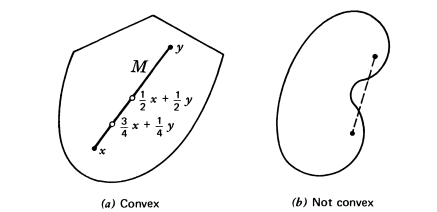
\includegraphics[scale=.7]{p65ex11.png} 
\\ \\
Let, $x,y \in \tilde{B}(0;1)$ which implies that $||x|| \le 1$ and $||y|| \le 1$.  Given any point $m \in M$ there exists $\alpha$ where $0\le \alpha \le 1$, such that $m=\alpha x + (1-\alpha)y$.  Thus, $||m|| = ||\alpha x + (1-\alpha)y||$
\begin{align*}
	\NORM{m} &= \NORM{\alpha x + (1-\alpha)y} \\
		&\le ||\alpha x|| + ||(1-\alpha)y||\\
		&\le |\alpha| \, ||x|| + |1-\alpha| \, ||y|| \\
	\text{Let } p &= \max(||x||,||y||) \\
	||m|| &\le |\alpha| \, p + |1-\alpha| \, p \\
		&\le (|\alpha| + |(1-\alpha)|)p \\
		&\le p \\
	\therefore m &\in \tilde{B}(0;1)
\end{align*}$x,y$ are arbitrary points and $m$ is an arbitrary point between them.  Hence, $\tilde{B}(0;1)$ must be convex.

\newpage
Page. 70 
\begin{enumerate}
	\item Show that $c \subset \ell^\infty$ is a vector space of $\ell^\infty$ (cf. 1.5-3) and so is $c_0$, the space of all sequences of scalars converging to zero.\\
	\\
	Given any $x,y \in \ell^\infty$ and $c_x, c_y$ are bounds for these sequences with $x = (\eta_j) \le c_x$ and $y=(\xi_j) \le c_y$.  Then given any $\alpha \in \C$ we have
	\begin{align*}
		\alpha(x + y) &= \alpha(\eta_j + \xi_j)_{j=1}^\infty & \text{component-wise addition} \\
		&= (\alpha\eta_j + \alpha\xi_j)_{j=1}^\infty \\
		|\alpha\eta_j + \alpha\xi_j|_{j=1}^\infty &\le |\alpha|(c_x + c_y)
	\end{align*}thus we have a new bounded sequence, that is $\alpha(x+y) \in \ell^\infty$.  Thus, $\ell^\infty$ is a vector space.\\ \\
	Notice that if $c_x = c_y = 0$ that $|\eta_j + \xi_j| \le c_x+c_y = 0$ for all $1 \le j < \infty$, thus $x+y \in c_0$.\\
	
	\item Show that $c_0$ in Prob 1 is a \textit{closed} subspace of $\ell^\infty$, so that $c_0$ is complete by 1.5-2 and 1.4-7. \\
	\\
	Let $x,y \in \ell^\infty \backslash c_0$ each converges to real numbers $c_x, c_y$, respectively.  Note that $c_x,c_y$ are strictly greater than zero.  Thus, $d(x,y) \le \max(c_x, c_y)$ and is distinctly not zero.  Hence, given any $\epsilon> 0$ there exists $B(x;\epsilon) \subset \ell^\infty\backslash c_0$.  Thus  $\ell^\infty\backslash c_0$ must be open which indicates that $c_0$ must be closed.\\
	
	\item In $\ell^\infty$, let $Y$ be the subset of all sequences with only finitely many nonzero terms.  Show that $Y$ is a subspace of $\ell^\infty$ but not a closed subspace. \\
	\\
	Let $x = (\eta_m), y=(\xi_m) \in \ell^\infty$ such that $I_x, I_y$ each represent a list of indices where $x_i \ne 0$ when $i \in I_x$ and similarly to $I_y$.  Then, we can see that $x+y$ will be the sequence $(z_m) = \PAREN{\eta_m + \xi_m}$.  We can see that when $j \in I_x \cup I_y$ that $z_j \ne 0$.  Hence, $I_z$ (the set of indices for non-zero entries in $z$) will be $I_z=I_x\cup I_y$.  Thus, $z \in Y$.  Given any $\alpha > 0$ we can see that it has no effect on $I_x$, thus $(\alpha \eta_m) \in Y$.  Since it is closed under addition and scalar multiplication it must be a vector space.\\
	\\
	Let $x_1= \{1,0,\dots \} \in Y$, that is, it has 1 in the first component.  And $x_2 = \{1,1,0\dots\}$ and so on.  The general term $x_i$ means that the first $i$ components are 1 and the remaining are zero.  Clearly, $x_i \in Y$ for all $i\in\N$.  However, the limit point of $x_i$ as $i$ increases without bound is $x_\infty=\{1, 1, \dots\}$ with one repeating forever.  $x_\infty \not \in Y$ hence a sequence in $Y$ does not contain its limit point which means that $Y$ is not closed.
	\\
	
	\setcounter{enumi}{7}
	\item If in a normed space $X$, absolute convergence of any series always implies convergence of that series, show that $X$ is complete.\\
	\\
	Suppose that $X$ is not complete.  Then there exists $x = (\eta_m) \in X$ that is an absolutely convergent series and converges but does NOT have a convergent subsequence.  That is, there exists a list of indices $\iota$ whose size is infinite, such that $\LIM{i\to\infty} \eta_{\iota_i} \ne 0$.  We know that given any $\epsilon > 0$ there exists an $N \in \N$ such that $|\eta_n - \eta_m| < \epsilon$ for all $n,m > N$.  Thus, we can pick indices for $\iota$, label them $\nu, \mu \in \N$ such that $\iota_\nu, \iota_\mu > N$ and hence $|\eta_{\iota_\nu}-\eta_{\iota_\mu}| < \epsilon$.  This means that $\LIM{i\to\infty} \eta_{\iota_i} = 0$ and $\eta_\iota$ is a subsequence that converges, hence $X$ must be complete.
	
	\item Show that in a Banach space, an absolutely convergent series is convergent.\\
	\\
	Let $x = (\eta_m) \in X$ be absolutely convergent.  Let $S_n = \SUM{i=1}{n} |\eta_i|$ be the partial sum of $x$.  There exists $\epsilon > 0$ and $N \in \N$ such that whenever $n > N, |S_n - S_\infty| < \epsilon$.  Let $m > n$ then 
	\begin{align*}
		|S_m - S_\infty| &< \epsilon \\
		|S_n - S_\infty| - |S_m - S_\infty| &< \epsilon \\
		|S_n - S_m| &< \epsilon
	\end{align*}WLOG let $m > n$ then
	\begin{align*}
		|S_n-S_m| &= \BARS{\sum_{i=1}^n |\eta_i| - \sum_{j=1}^m |\eta_j|} < \epsilon \\
		\therefore |\eta_n - \eta_m| &< \epsilon
	\end{align*}which implies that $x$ is convergent.
	
	\item \textbf{(Schauder basis)} Show that if a normed space has a Shauder basis, it is separable.\\
	\\
	\textbf{Shauder Basis implies Countable:} Let $\{ e_i \}_{i=1}^\infty$ be a Shauder Basis for the normed space $X$.  Then for any $x \in X$ there exists a unique sequence $(\alpha_m)$ such that $\BARS{x - \SUM{i=1}{n} \alpha_i e_i} \to 0$ as $n \to \infty$.  Clearly, $(\alpha_m)$ is countable.  Given any $x,y \in X$ then $x+y \in X$ and since both $x,y$ can be made up countable sequences so can $x+y$, further there may not exist a $z$ with and uncountable sequences, meaning that the Shauder Basis doesn't span $X$.\\ \\
	\textbf{Shauder Basis implies dense:}  Let $x,y \in X$ such that $|x-y|<\epsilon$ for some $\epsilon > 0$.  Then $\exists! (\alpha_m)$ and $\exists! (\beta_m)$ such that $\BARS{x - \SUM{i=1}{n} \alpha_i e_i} \to 0$ and $\BARS{y - \SUM{i=1}{n} \beta_i e_i} \to 0$ as $n \to \infty$ and we can say
	\begin{align*}
		x &= \SUM{i=1}{\infty} \alpha_i e_i \text{ and } y = \SUM{i=1}{\infty} \beta_i e_i\\
		\text{Let } \gamma_i &= \frac{\alpha_i + \beta_i}{2}, \, \forall i \in \N \\
		z &= \SUM{i=1}{n} \gamma_i e_i 
	\end{align*}Note that
	\begin{align*}
		z &= \SUM{i=1}{\infty} \frac{\alpha_i + \beta_i}{2} \\
		2z &= \SUM{i=1}{\infty}\PAREN{ \alpha_i + \beta_i } \\
		2z &= x+y \\
		2|| z || &\le ||x||+||y||
	\end{align*}and 
	\begin{align*}	
		|| z || &\ge c\sum_{i=1}^\infty | \gamma_i| \\
			&\ge c\sum_{i=1}^\infty \BARS{\frac{\alpha_i + \beta_i}{2}} \\
			&\ge c\sum_{i=1}^\infty \frac{|\alpha_i| + |\beta_i|}{2} \\
			&\ge \frac{c}{2} \PAREN{\sum_{i=1}^\infty |\alpha_i| + \sum_{i=1}^\infty|\beta_i| } \\
		2|| z|| &\ge ||x|| + ||y|| \\
	\end{align*} therefore $2||z||=||x|| + ||y||$ and between $||x||$ and $||y||$ ($||z||$ is the average of the other norms of the other two vectors).  Thus, given any two vectors within $X$ there is a vector between them which means that $X$ is dense.
	
	\item Show that $(e_n)$, where $e_n=(\delta_{nj})$, is a Schauder basis for $\ell^p$, where $1 \le p < +\infty$.\\
	\\
	\textbf{Span of $(e_n)$:}  Let $x=\{ x_1, x_2, x_3, \dots \} \in X$.  We can see that
	\begin{align*}
		\begin{array}{cccccc}
			e_1 = \{ & 1, & 0, & 0, & \cdots & \} \\
			e_2 = \{ & 0, & 1, & 0, & \cdots  &\} \\
			e_3 = \{ & 0, & 0, & 1, & \cdots  &\} \\
			\vdots \\
			x = & x_1 e_1 + & x_2 e_2 + & x_3 e_3 + & \cdots
		\end{array}
	\end{align*}thus span$(\,(e_n)\,)= \ell^p$.\\
	\textbf{Uniqueness of coordinates:}  Let us suppose that there exists a sequence $( \alpha_i )$ such that $\alpha_i \ne x_i$ for some values for $i$ and $x = (\alpha_i)$.  Since, the $d(\,(\alpha_n),(x_m)\,)=0$ since
	\begin{align*}
		||x|| &= \PAREN{\sum_{i=1}^\infty |x_i|^p}^{1/p} \\
		|| (\alpha_n) - (x_n) || &= \PAREN{\sum_{i=1}^\infty |\alpha_i e_i - x_i e_i|^p}^{1/p} \\
			&= \PAREN{\sum_{i=1}^\infty (|\alpha_i - x_i| e_i)^p}^{1/p} =0
	\end{align*}each $e_i$ is a constant sequence and each $|\alpha_i - x_i| \ge 0$.  Which implies that $|\alpha_i - x_i|=0$ for all $i=1, \dots, \infty$. Hence, all it must be that $\alpha_i = x_i$ for all $i$ and the coordinates are unique.
	
	\setcounter{enumi}{14}
	\item \textbf{(Product of normed spaces)}  If $(X_1,||\cdot||_1)$ and $(X_2, ||\cdot||_2)$ are normed spaces, show that the product vector space $X=X_1\times X_2$ (cf. prob 13, Sec 2.1) becomes a normed space if we define
	\begin{align*}
		 ||x||=\max\PAREN{||x_1||_1, ||x_2||_2} \text{ where } x=(x_1, x_2).
	\end{align*}
	
	We must show that this defintion of $\NORM{x}$ has all of the properties that define a norm.
	\begin{itemize}
		\item Is $\NORM{x} \ge 0$?
		
		Since both $\NORM{x_1}_1 \ge 0$ always and $\NORM{x_2}_2 \ge 0$ always then $\max\PAREN{\NORM{x_1}_1, \NORM{x_2}_2} \ge 0$ always.
		
		\item Does $\NORM{x} = 0$ imply that $x=0$?

		If either $\NORM{x_1}_1 \ne 0$ or $\NORM{x_2}_2 \ne 0$ (but not both) implies that $\NORM{x} > 0$ then the only condition where $\NORM{x}=0$ is when they are both zero.  Thus $x = (0,0)$.
		
		\item Is it true that $\NORM{\alpha x} = |\alpha| \NORM{x}$ for all $\alpha \in K$?
		
		$\alpha x = (\alpha x_1, \alpha x_2)$ thus 
		\begin{align*}
			\NORM{\alpha x} &= \max\PAREN{\NORM{\alpha x_1}_1, \NORM{\alpha x_2}_2} \\
				&= \max\PAREN{|\alpha|\NORM{ x_1}_1, |\alpha|\NORM{x_2}_2} \\
				&= |\alpha|\max\PAREN{\NORM{ x_1}_1, \NORM{x_2}_2}  \\
				&= |\alpha|\NORM{x}
		\end{align*}		  
		
		\item Is the Triangular Inequality true for any two vectors?
		
		Given any $x=(x_1, x_2),y=(y_1,y_2) \in X_1 \times X_2$
		\begin{align*}
			\NORM{x+y} &= \NORM{(x_1, x_2)+(y_1,y_2)} \\
				&= \NORM{\PAREN{x_1+y_1, x_2+y_2 }} \\
				&= \max\PAREN{\NORM{x_1+y_1}, \NORM{x_2+y_2} }\\
				&\le \max\PAREN{\NORM{x_1}+\NORM{y_1}, \NORM{x_2}+\NORM{y_2} }\\
				&\le \max(\NORM{x_1},\NORM{x_2}) + \max(\NORM{y_1}, \NORM{y_2}) \\
				&\le \NORM{x} + \NORM{y}
		\end{align*}
	\end{itemize}
\end{enumerate}

\newpage

Page. 76 \#1.  Give examples of subspaces of $\ell^\infty$ and $\ell^2$ which are not closed.\\
\\
Let $X \subset \ell^\infty$ such that each sequence has finitely many non-zero elements unioned with the zero sequence.  Any two such sequences added together will be another sequence of the same type, thus closed under addition.  So, too, with scalar multiplication.  However, if we define $x_1 = \{1, 0, \dots \},$ $x_2 = \{1,1,0,\dots \}$, $x_3=\{1,1,1,0,\dots\}$ and so on.  $\LIM{n\to \infty} x_n = \{1,1,1,\dots\} \not \in X$.  Hence, there exists a sequence in $X$ where $X$ does not contain its limit point.  The same is true if $X \subset \ell^2$.


\end{document}